% Taxonomy Diagram — Standalone TikZ
% Compile: pdflatex taxonomy_diagram_tikz.tex
% Then include in main survey with 
\includegraphics{figures/taxonomy_diagram.pdf}

\documentclass[tikz,border=4pt]{standalone}
\usepackage{tikz}
\usetikzlibrary{shapes.geometric,arrows.meta,positioning,fit,backgrounds,shadows}

\definecolor{cblue}{HTML}{003f87}
\definecolor{cred}{HTML}{c0392b}
\definecolor{cgreen}{HTML}{1a7a4a}
\definecolor{corange}{HTML}{e67e22}
\definecolor{cgray}{HTML}{7f8c8d}
\definecolor{cpurple}{HTML}{8e44ad}
\definecolor{lcyan}{HTML}{d6eaf8}
\definecolor{lgreen}{HTML}{d5f5e3}
\definecolor{lorange}{HTML}{fdebd0}

\tikzset{
  L1node/.style={
    rectangle, rounded corners=4pt, draw=cblue, fill=cblue!15,
    text width=2.1cm, align=center, font=\small\bfseries,
    minimum height=0.8cm, drop shadow
  },
  L2node/.style={
    rectangle, rounded corners=3pt, draw=cgreen!70!black, fill=lgreen,
    text width=1.8cm, align=center, font=\scriptsize,
    minimum height=0.65cm
  },
  L3node/.style={
    ellipse, draw=corange!80!black, fill=lorange,
    text width=1.5cm, align=center, font=\tiny,
    minimum height=0.5cm
  },
  arrow/.style={-{Latex[length=2mm]}, thick, color=cgray},
  label/.style={font=\footnotesize\bfseries, color=cblue}
}

\begin{document}
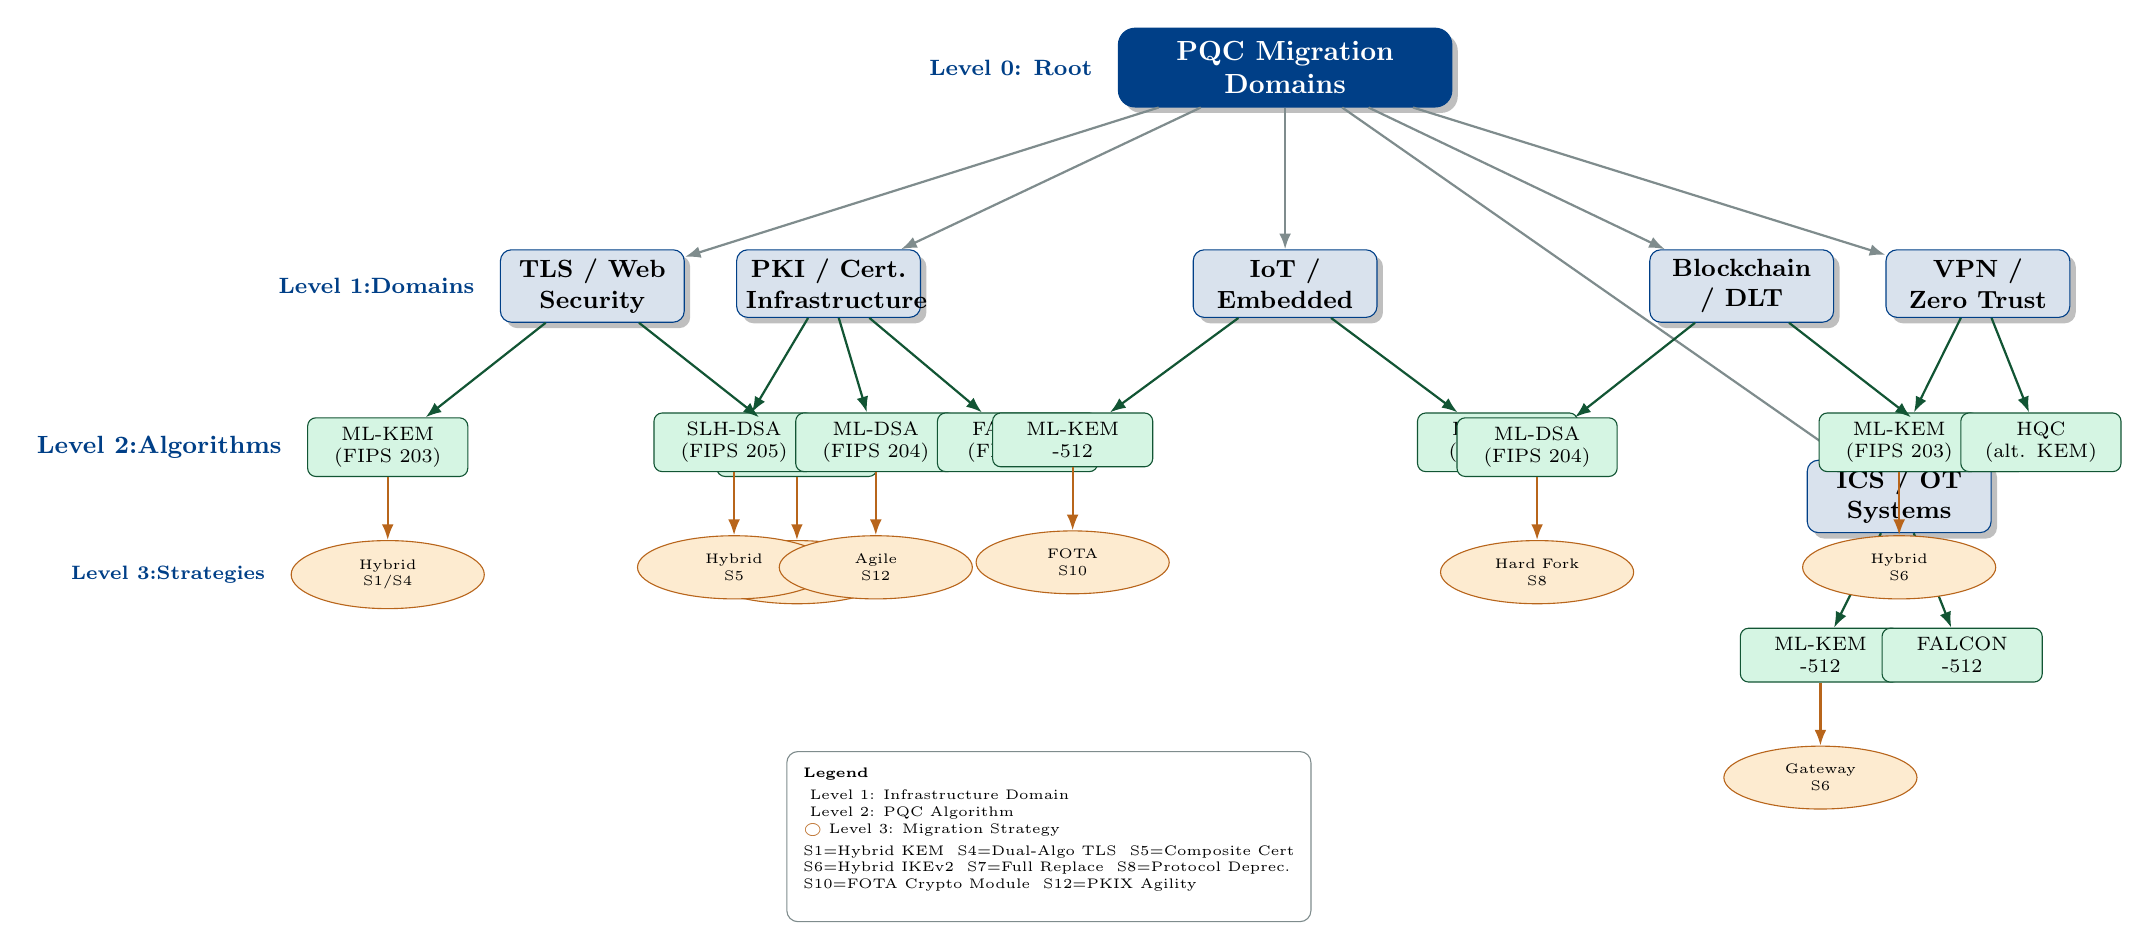
\begin{tikzpicture}[node distance=0.4cm and 0.5cm]

%── LEVEL 1 ROOT ─────────────────────────────────────────────────────────────
\node[rectangle, rounded corners=6pt, draw=cblue, fill=cblue, text=white,
      text width=4.0cm, align=center, font=\normalsize\bfseries,
      minimum height=1.0cm, drop shadow] (root)
  {PQC Migration\\Domains};

%── LEVEL 1 DOMAIN NODES ─────────────────────────────────────────────────────
\node[L1node, below left=1.8cm and 5.5cm of root]  (tls)  {TLS / Web\\Security};
\node[L1node, below left=1.8cm and 2.5cm of root]  (pki)  {PKI / Cert.\\Infrastructure};
\node[L1node, below=1.8cm of root]                 (iot)  {IoT /\\Embedded};
\node[L1node, below right=1.8cm and 2.5cm of root] (bcn)  {Blockchain\\/ DLT};
\node[L1node, below right=1.8cm and 5.5cm of root] (vpn)  {VPN /\\Zero Trust};

%── ICS separate (wider spacing) ─────────────────────────────────────────────
\node[L1node, below=1.8cm of vpn, xshift=-1.0cm]   (ics)  {ICS / OT\\Systems};

%── Domain arrows from root ───────────────────────────────────────────────────
\foreach \d in {tls,pki,iot,bcn,vpn}
  \draw[arrow] (root) -- (\d);
\draw[arrow] (root) -- (ics);

%── LEVEL 2 ALGORITHM NODES ──────────────────────────────────────────────────
% TLS
\node[L2node, below left=1.2cm and 0.4cm of tls]  (mlkem-tls)  {ML-KEM\\(FIPS 203)};
\node[L2node, below right=1.2cm and 0.4cm of tls] (mldsa-tls)  {ML-DSA\\(FIPS 204)};

% PKI
\node[L2node, below=1.2cm of pki, xshift=-1.2cm]  (slhdsa-pki) {SLH-DSA\\(FIPS 205)};
\node[L2node, below=1.2cm of pki, xshift=0.6cm]   (mldsa-pki)  {ML-DSA\\(FIPS 204)};
\node[L2node, below=1.2cm of pki, xshift=2.4cm]   (falcon-pki) {FALCON\\(FN-DSA)};

% IoT
\node[L2node, below left=1.2cm and 0.5cm of iot]  (mlkem-iot)  {ML-KEM\\-512};
\node[L2node, below right=1.2cm and 0.5cm of iot] (falcon-iot) {FALCON\\(compact)};

% Blockchain
\node[L2node, below left=1.2cm and 0.4cm of bcn]  (mldsa-bcn)  {ML-DSA\\(FIPS 204)};
\node[L2node, below right=1.2cm and 0.4cm of bcn] (slhdsa-bcn) {SLH-DSA\\-128f};

% VPN
\node[L2node, below=1.2cm of vpn, xshift=-1.0cm]  (mlkem-vpn)  {ML-KEM\\(FIPS 203)};
\node[L2node, below=1.2cm of vpn, xshift=0.8cm]   (hqc-vpn)    {HQC\\(alt. KEM)};

% ICS
\node[L2node, below=1.2cm of ics, xshift=-1.0cm]  (mlkem-ics)  {ML-KEM\\-512};
\node[L2node, below=1.2cm of ics, xshift=0.8cm]   (falcon-ics) {FALCON\\-512};

% Draw L1->L2 arrows
\foreach \d/\alg in {tls/mlkem-tls, tls/mldsa-tls, pki/slhdsa-pki, pki/mldsa-pki, pki/falcon-pki,
                      iot/mlkem-iot, iot/falcon-iot, bcn/mldsa-bcn, bcn/slhdsa-bcn,
                      vpn/mlkem-vpn, vpn/hqc-vpn, ics/mlkem-ics, ics/falcon-ics}
  \draw[arrow, color=cgreen!70!black] (\d) -- (\alg);

%── LEVEL 3 STRATEGY NODES ────────────────────────────────────────────────────
\node[L3node, below=0.8cm of mlkem-tls] (hyb-tls) {Hybrid\\S1/S4};
\node[L3node, below=0.8cm of mldsa-tls] (full-tls) {Full Rep.\\S7};
\node[L3node, below=0.8cm of slhdsa-pki] (hyb-pki) {Hybrid\\S5};
\node[L3node, below=0.8cm of mldsa-pki]  (agile-pki) {Agile\\S12};
\node[L3node, below=0.8cm of mlkem-iot]  (ota-iot) {FOTA\\S10};
\node[L3node, below=0.8cm of mldsa-bcn]  (fork-bcn) {Hard Fork\\S8};
\node[L3node, below=0.8cm of mlkem-vpn]  (hyb-vpn) {Hybrid\\S6};
\node[L3node, below=0.8cm of mlkem-ics]  (gw-ics)  {Gateway\\S6};

\foreach \alg/\strat in {mlkem-tls/hyb-tls, mldsa-tls/full-tls, slhdsa-pki/hyb-pki,
                          mldsa-pki/agile-pki, mlkem-iot/ota-iot, mldsa-bcn/fork-bcn,
                          mlkem-vpn/hyb-vpn, mlkem-ics/gw-ics}
  \draw[arrow, color=corange!80!black] (\alg) -- (\strat);

%── Legend ────────────────────────────────────────────────────────────────────
\node[below=5.5cm of iot, xshift=-3cm,
      rectangle, draw=cgray, fill=white, rounded corners=4pt,
      inner sep=6pt, font=\tiny, align=left]
  (legend) {
    \textbf{Legend}\\[2pt]
    {\color{cblue}$\blacksquare$} Level 1: Infrastructure Domain\\
    {\color{cgreen!70!black}$\blacksquare$} Level 2: PQC Algorithm\\
    {\color{corange!80!black}$\bigcirc$} Level 3: Migration Strategy\\[2pt]
    S1=Hybrid KEM\ \ S4=Dual-Algo TLS\ \ S5=Composite Cert\\
    S6=Hybrid IKEv2\ \ S7=Full Replace\ \ S8=Protocol Deprec.\\
    S10=FOTA Crypto Module\ \ S12=PKIX Agility\\
  };

%── Level Labels ──────────────────────────────────────────────────────────────
\node[label, left=0.2cm of root]    {Level 0: Root};
\node[label, left=0.2cm of tls]     {Level 1:\\Domains};
\node[label, left=0.2cm of mlkem-tls] {\small Level 2:\\Algorithms};
\node[label, left=0.2cm of hyb-tls]   {\scriptsize Level 3:\\Strategies};

\end{tikzpicture}
\end{document}
